\definecolor{genecolor}{RGB}{94,135,173}

\section*{Motivations}

\begin{frame}
  \frametitle{Statistical analysis of Networks}
  \framesubtitle{Different questions}

  \begin{block}{Understanding the network topology}
    \vspace{-.25cm}
    \begin{itemize}
    \item Data = observed network
    \item Questions: central nodes? cluster structure? small-world property?
    \end{itemize}
  \end{block}
  
  \vfill

  \begin{alertblock}{Inferring/Reconstructing the network}
    \vspace{-.25cm}
    \begin{itemize}
    \item Data = repeated signal observed at each node
    \item Questions: which nodes are connected?
    \end{itemize}
  \end{alertblock}

  \vfill

  \begin{block}{Using the network}
    \vspace{-.25cm}
    \begin{itemize}
    \item Data = a given network + signal on nodes
    \item Questions: how the epidemic spreads along the network?
    \end{itemize}
  \end{block}

  \vfill

  \begin{block}{\alert{Each to be combined with}}
    covariates, time, heterogeneous data set, missing data, ...  
  \end{block}
\end{frame}

\begin{frame}
  \frametitle{Automatic reconstruction of biological networks (1)} 
  \framesubtitle{E. coli regulatory network}  

  \begin{columns}
    \begin{column}{.4\textwidth}
      \begin{small}
        \begin{block}{Target network}
          Relations between genes and their products
          \begin{itemize}
          \item highly structured
          \item always incomplete
          \end{itemize}
        \end{block}
      \end{small}
      \begin{small}
        \begin{block}{Data and method}
          \begin{itemize}
          \item transcriptomic data
          \item Gaussian graphical model with sparse methods
          \end{itemize}
        \end{block}
      \end{small}
    \end{column}
    \begin{column}{.55\textwidth}
      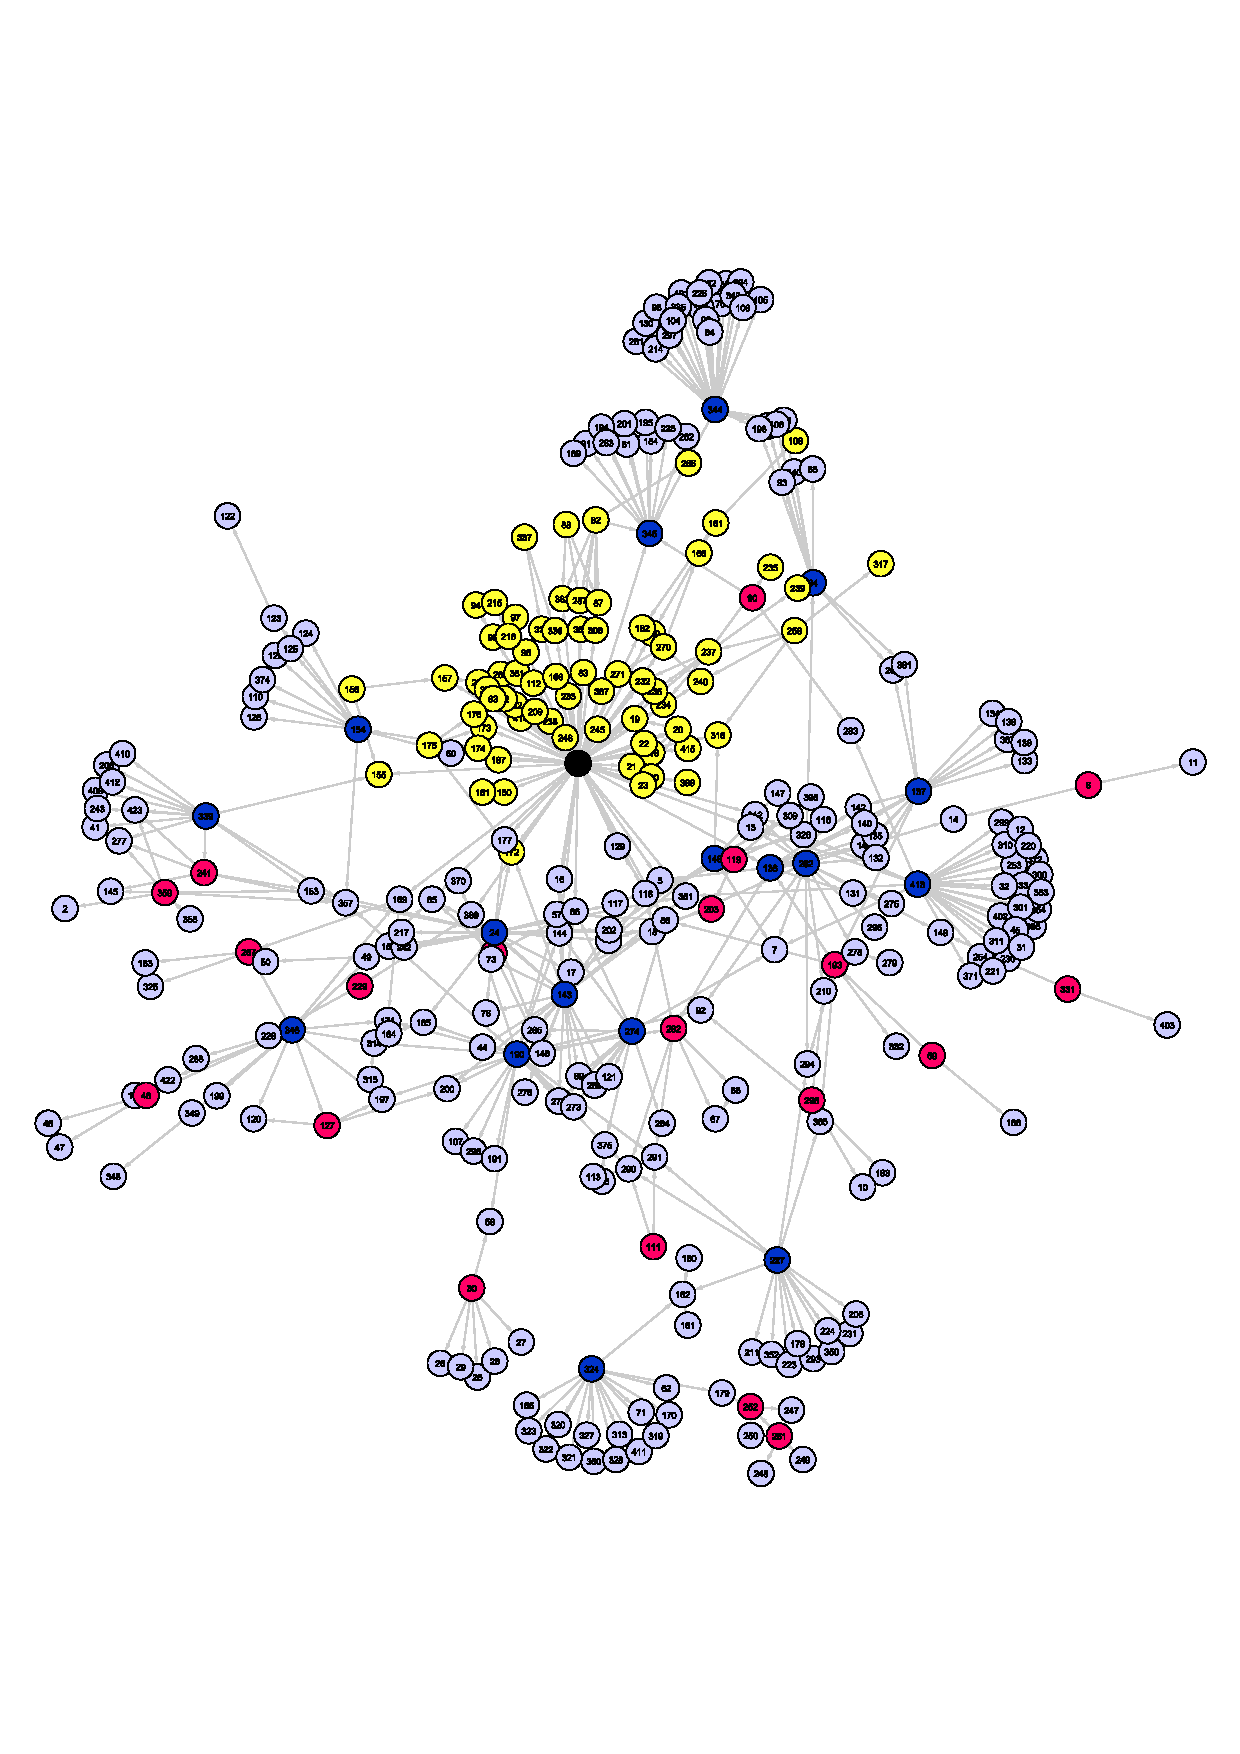
\includegraphics[width=\textwidth]{figures/net_reg_ecoli}
    \end{column}
  \end{columns}
\end{frame}

\begin{frame}
  \frametitle{Automatic  reconstruction  of biological  networks  (2)}
  \framesubtitle{Microbial  association   network  of  the   oak  tree susceptible to the foliar fungal pathogen}

  \begin{columns}
    \begin{column}{.4\textwidth}
      \begin{small}
        \begin{block}{Target network}
          Relations between microbial species (bacterial or fungal)
          \begin{itemize}
          \item highly structured
          \item represents co-abudancies
          \end{itemize}
        \end{block}
      \end{small}
      \begin{small}
        \begin{block}{Data and method}
          \begin{itemize}
          \item OTUs table/abundances
          \item correlation + test/threshold
          \end{itemize}
        \end{block}
      \end{small}
    \end{column}
    \begin{column}{.55\textwidth}
      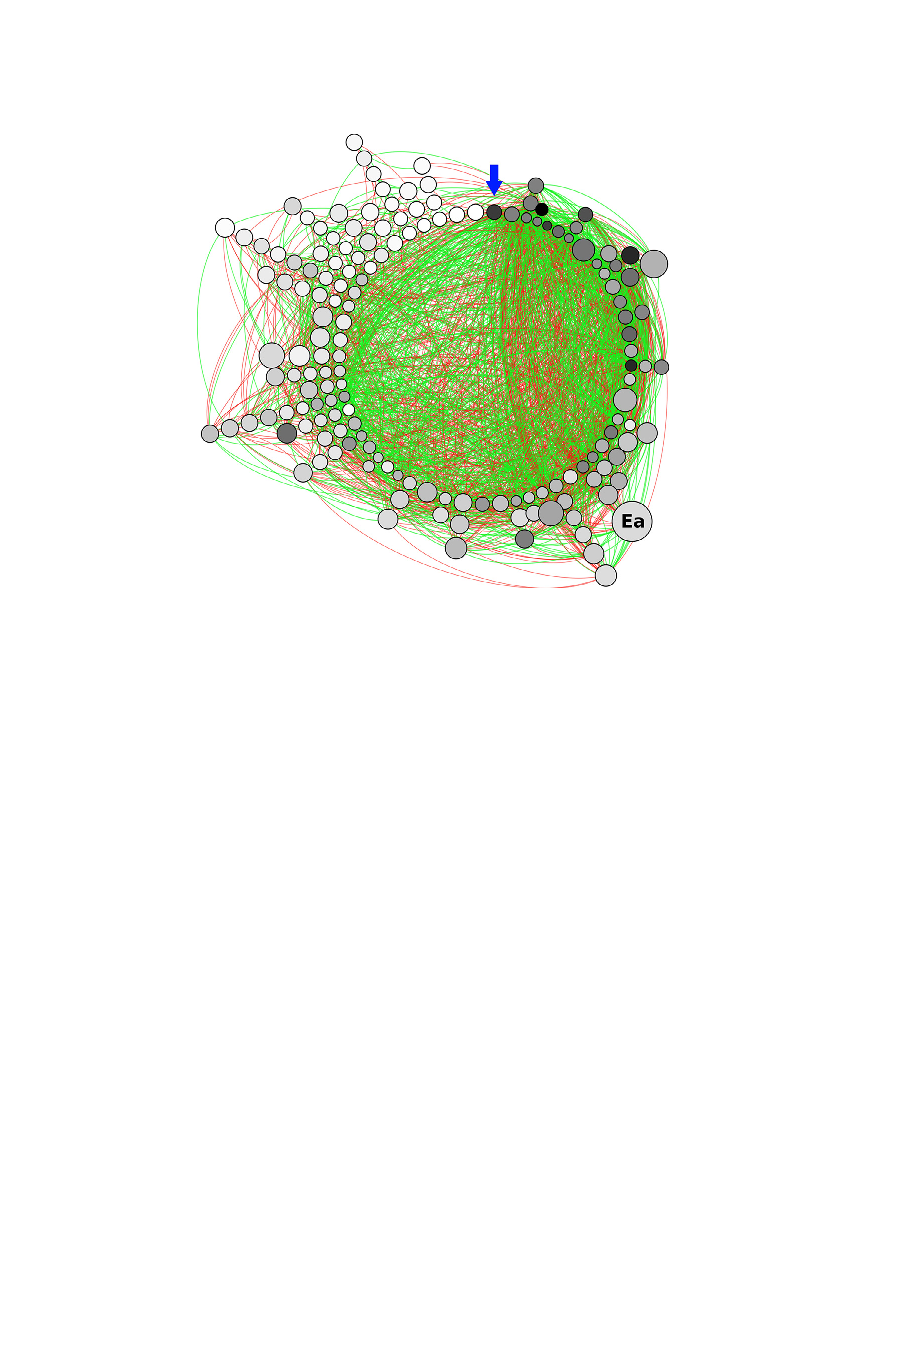
\includegraphics[width=\textwidth]{figures/cor_net_eco}
      \begin{scriptsize}
         Vacher et al., Advances in Ecological Research
      \end{scriptsize}
    \end{column}
  \end{columns}

\end{frame}

\begin{frame}
  \frametitle{A challenging problem}

  \begin{columns}[c]
    \begin{column}{.55\textwidth}
      \begin{tikzpicture}[scale=0.75]
        \node[scale=0.75,opacity=0.75] at (-3,3) {\pgfuseimage{sequencer}};
        \node[scale=0.75] at (-3.5,1) {\pgfuseimage{affymetrix}};
        \node[scale=0.75,fill=red, text=white,single arrow] 
        (inference) at (-1.7,1.7) {\sf \scriptsize Inference}; 
        
        \node at (-3,-0.5) {\begin{tabular}{@{}c@{}}
            \tiny $\approx$ 10s/1,000s assays \\ 
            \tiny $\approx $ 1,000s/1,000,000s features \\
          \end{tabular}
        };
        
        %% UN GRAPH 
        \tikzstyle{every edge}=[-,>=stealth',shorten >=1pt,auto,thin,draw,color=genecolor]
        \tikzstyle{every node}=[fill=genecolor]
        \tikzstyle{every state}=[draw=none,text=white,scale=0.5, transform shape] 
        
        % premier cluster
        \node[state] (A1) at (0,1.75) {g1};
        \node[state] (A2) at (1,0.75) {g2};
        \node[state] (A3) at (0,-.25) {g3};
        \node[state] (A4) at (-1,0.75) {g4};
        \node[state] (A5) at (0,0.75) {g5};
        
        \foreach   \name/\angle/\text   in  {B1/234/g6,   B2/162/g7,
          B3/90/g8, B4/18/g9, B5/-54/g10} {
          \node[state,xshift=4cm,yshift=4cm]     (\name)    at
          (\angle:1cm) {\text}; }
        
        \node[state] (B6) at (2,2) {g11};
        \node[state] (C1) at (3,0.5) {g12};
        \node[state] (C2) at (2.2,0) {g13};
        
        \path 
        (A5) edge [bend left] (A1)
        (A5) edge [bend left] (A2)
        (A5) edge [bend left] (A3)
        (A5) edge [bend left] (A4)
        (B6) edge [bend right] (B1) 
        (B6) edge [bend right] (B2) 
        (B6) edge [bend right] (B3) 
        (B6) edge [bend right] (B4) 
        (B6) edge [bend right] (B5) 
        (C2) edge [bend left] (C1)
        (A5) edge [bend left] (B6)
        (B6) edge [bend right] (C2);
      \end{tikzpicture}
    \end{column}
    \begin{column}{.475\textwidth} 
      \begin{block}{Model point of view}
        \vspace{-.25cm}
        \begin{footnotesize}
            \begin{enumerate}
            \item \alert{Nodes} (genes, OTUS, ...)
              \begin{scriptsize}
                \begin{itemize}
                \item \scriptsize fixed variables
                \end{itemize}
              \end{scriptsize}
            \item \alert{Edges} (biological interactions)
              \begin{scriptsize}
                \begin{itemize}
                \item \scriptsize use (partial) correlations or others
                  fancy statistical concepts
                \end{itemize}
              \end{scriptsize}
            \item \alert{Data} (intensities, counts)
              \begin{scriptsize}
                \begin{itemize}
                \item \scriptsize a tidy $n\times p$ dat matrix
                \end{itemize}
              \end{scriptsize}
            \end{enumerate}
            \vspace{-.25cm}
            $\rightsquigarrow$ \alert{Quantities and goals well defined}
          \end{footnotesize}
          \end{block}
    \end{column}
  \end{columns}

  \vspace{-.25cm}
  \begin{block}{Data point of view: \alert{non classical statistics}}<2->
    \vspace{-.25cm}
    \begin{footnotesize}
    \begin{itemize}
    \item (Ultra) High dimensionality ($n<p$, $n\lll p$)
    \item Heterogeneous data
    \end{itemize}
      \end{footnotesize}    
  \end{block}
  \vspace{-.35cm}
  \begin{block}{Biological point of view: \alert{not well defined goals and questions}}<2>
    \vspace{-.25cm}    
    \begin{footnotesize}
    \begin{itemize}
    \item What interaction? Direct? Indirect? Causal?
    \item Whole network? Subnetwork? Groups of key actors?
    \end{itemize}
      \end{footnotesize}    
  \end{block}

\end{frame}

